\documentclass[12pt, a4paper]{article}

\usepackage[a4paper, top=2.5cm, bottom=2.5cm, left=2.5cm, right=2.5cm]{geometry}
\usepackage{graphicx}
\usepackage{amsmath}
\usepackage{amssymb}
\usepackage{float}
\usepackage{booktabs}
\usepackage{parskip}
\usepackage{siunitx}
\usepackage{enumitem}
\usepackage[hidelinks]{hyperref}
\usepackage{titlesec}
\usepackage{fancyhdr}

\pagestyle{fancy}
\fancyhf{}
\rhead{42059/41034 --- Lab 2}
\lhead{CMOS Inverter}
\cfoot{\thepage}

\titleformat{\section}{\large\bfseries}{}{0em}{}[\titlerule]
\titleformat{\subsection}{\normalsize\bfseries}{}{0em}{}

\graphicspath{{drive-download-20260305T060328Z-1-001/}}
\usepackage{grffile}

\begin{document}

\begin{titlepage}
    \centering
    \vspace*{2cm}
    {\LARGE\bfseries 42059 / 41034 --- Lab 2 Report\par}
    \vspace{0.5cm}
    {\Large CMOS Inverter\par}
    \vspace{1.5cm}
    \begin{tabular}{rl}
        \textbf{Student Name:} & Nathan Nguyen       \\[0.4em]
        \textbf{Student ID:}   & 24493999         \\[0.4em]
        \textbf{Session:}      & Autumn 2026  \\[0.4em]
        \textbf{Date:}         & 5 March 2026 \\
    \end{tabular}
    \vfill
    {\small University of Technology Sydney}
\end{titlepage}

%------------------------
\section{Exercise 1: Transient Analysis}
%------------------------

\begin{figure}[H]
    \centering
    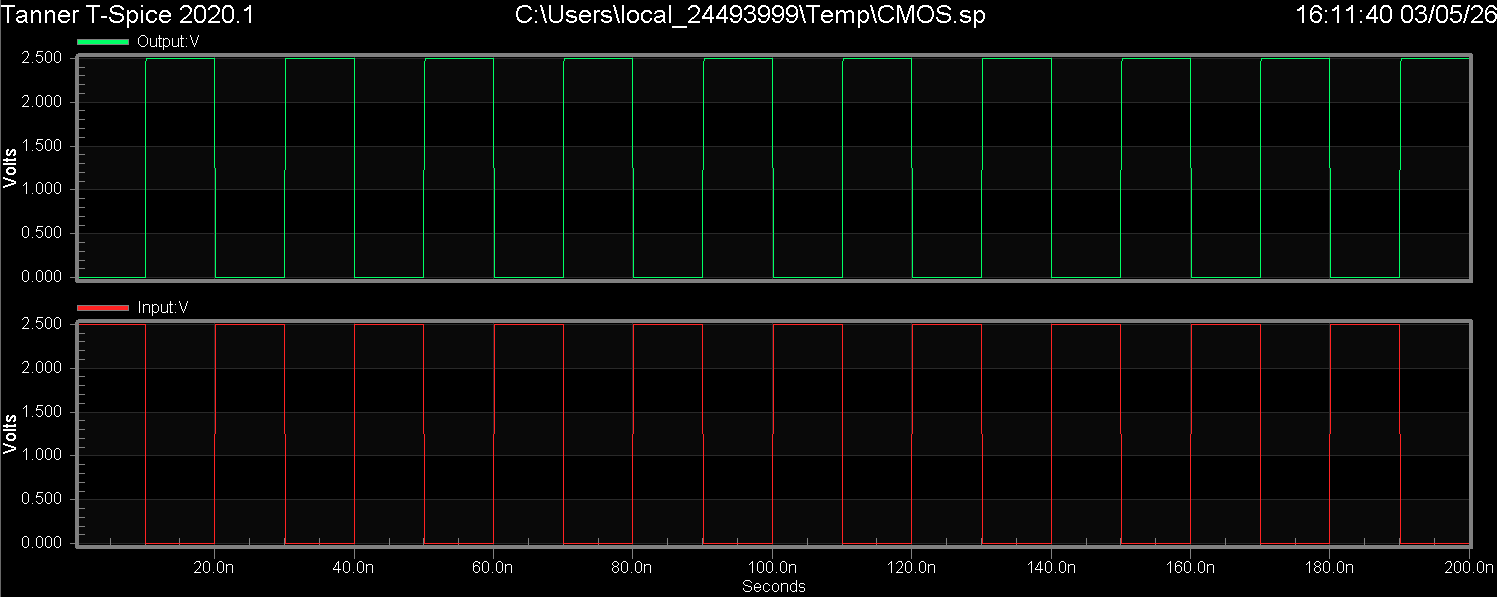
\includegraphics[width=\textwidth]{lab2.1}
    \caption{Transient simulation of the CMOS inverter. Output (green) is the logic complement of the input (red), confirming NOT gate operation with full rail-to-rail swing.}
    \label{fig:transient}
\end{figure}

\begin{table}[H]
    \centering
    \caption{Measured rise and fall times at the inverter output.}
    \begin{tabular}{lcc}
        \toprule
        \textbf{Parameter} & \textbf{Measure Name} & \textbf{Value} \\
        \midrule
        Rise time ($t_r$) & MeasureRiseTime\_1  & [value]\,ps \\
        Fall time ($t_f$) & MeasureFallTime\_1  & [value]\,ps \\
        \bottomrule
    \end{tabular}
\end{table}

Rise time is longer than fall time because the NMOS discharges the output faster than the PMOS charges it ($\mu_n > \mu_p$). The output is a phase-inverted replica of the input: when $V_\mathrm{in}$ is high, only the NMOS is ON and pulls the output to GND; when $V_\mathrm{in}$ is low, only the PMOS is ON and pulls the output to $V_\mathrm{DD}$. No static current flows in either steady state, so static power dissipation is zero.

%------------------------
\section{Exercise 2: Static Analysis}
%------------------------

\begin{figure}[H]
    \centering
    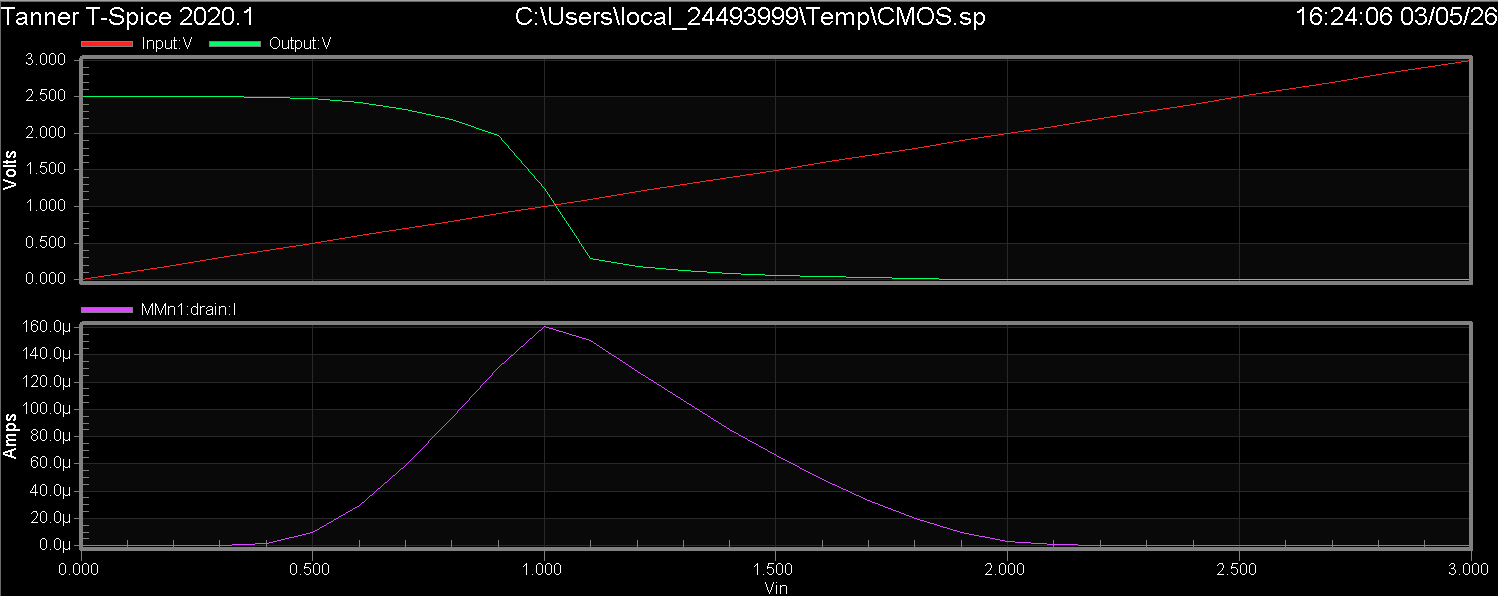
\includegraphics[width=\textwidth]{lab2.2}
    \caption{DC sweep results. Top: VTC showing $V_M \approx 0.9$--$1.0$\,V. Bottom: drain current peak ($\approx 160\,\mu$A) at the switching threshold, where both transistors partially conduct simultaneously.}
    \label{fig:static}
\end{figure}

\subsection{Switching Threshold and Skewness}

The VTC is skewed left: $V_M \approx 0.9$--$1.0$\,V vs.\ the ideal $V_\mathrm{DD}/2 = 1.25$\,V.

This is caused by the Beta ratio $\beta < 1$. With equal transistor dimensions, $\beta = \mu_p/\mu_n \approx 0.25$--$0.4$, so the NMOS is stronger and pulls the threshold below the midpoint. Substituting into
\[
    V_M = \frac{V_\mathrm{Tn} + \sqrt{\beta}\,(V_\mathrm{DD} - |V_\mathrm{Tp}|)}{1 + \sqrt{\beta}}
\]
with $\beta \approx 0.25$, $V_\mathrm{Tn} = |V_\mathrm{Tp}| = 0.5$\,V gives $V_M \approx 1.0$\,V, consistent with the simulation.

\subsection{Maximum Power Consumption}

Peak instantaneous power occurs at the switching threshold where both transistors partially conduct (crowbar current):
\[
    P_\mathrm{peak} = I_\mathrm{DS,peak} \times V_\mathrm{DD} \approx 160\,\mu\mathrm{A} \times 2.5\,\mathrm{V} = 400\,\mu\mathrm{W}
\]

\subsection{Correcting the Skew ($\beta = 1$)}

Increasing the PMOS width compensates for lower hole mobility:
\[
    W_p = \frac{\mu_n}{\mu_p} \cdot W_n \approx 2.5 \times 1.5\,\mu\mathrm{m} \approx 3.75\,\mu\mathrm{m}
\]
After this change, the VTC becomes symmetric about $V_\mathrm{DD}/2 = 1.25$\,V.

%------------------------
\section{Exercise 3: Inverter Layout}
%------------------------

\begin{figure}[H]
    \centering
    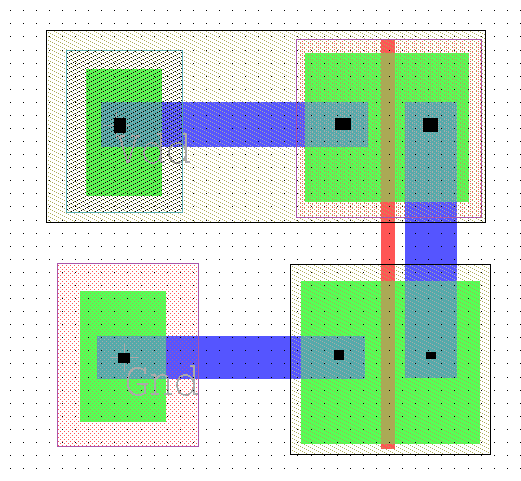
\includegraphics[width=0.72\textwidth]{lab2.3}
    \caption{Completed CMOS inverter layout. PMOS (top) is enclosed in the N-Well. NMOS (bottom) sits in the P-substrate. Shared Poly gate forms the \textsc{Input}; Metal1 connects both drains as \textsc{Output}.}
    \label{fig:layout}
\end{figure}

\begin{table}[H]
    \centering
    \caption{Terminal identification for the inverter layout.}
    \begin{tabular}{llll}
        \toprule
        \textbf{Terminal} & \textbf{Device} & \textbf{Layer} & \textbf{Connection} \\
        \midrule
        Gate (G)      & PMOS \& NMOS & Poly   & \textsc{Input} (shared) \\
        Drain (D)     & PMOS \& NMOS & Metal1 & \textsc{Output} (shared) \\
        Source (S)    & PMOS         & Metal1 & VDD \\
        Source (S)    & NMOS         & Metal1 & GND \\
        Body (B)      & PMOS         & N-Well & VDD via N-Implant contact \\
        Body (B)      & NMOS         & P-sub  & GND via P-Implant contact \\
        \bottomrule
    \end{tabular}
\end{table}

\subsection{Modifying Layout for $\beta = 1$}

Widen the PMOS active region from $\approx 1.5\,\mu$m to $\approx 3.75\,\mu$m (extend N-Well, P-Implant, Active, Metal1, and Poly gate width accordingly). NMOS dimensions are unchanged.

\subsection{Alternative Layout Topologies}

\begin{enumerate}
    \item \textbf{Standard cell (used here):} PMOS above NMOS, horizontal power rails, vertical Poly gate. Used in all modern digital cell libraries.
    \item \textbf{Folded/interdigitated:} Channel split into multiple fingers in parallel. Reduces gate resistance; used in RF/high-speed circuits.
    \item \textbf{Abutted cells:} Adjacent cells share diffusion regions, eliminating redundant contacts and reducing area.
    \item \textbf{FinFET (sub-22\,nm):} 3D transistors where width is set by discrete fin count rather than a continuous planar dimension.
\end{enumerate}

\end{document}